% TU/e Style Master Thesis template for LaTeX.

\documentclass[a4paper,10pt,twoside]{report}

% Packages are defined at the thesis.sty file.
\usepackage{thesis}

% Define key:value pairs.
\newcommand{\shortdoctitle}{Internship report}
\newcommand{\doctitle}{GPGPU acceleration}
\newcommand{\docsubtitle}{Internship report}
\newcommand{\me}{Lucas Bekker}
\newcommand{\keywords}{GPGPU}
\newcommand{\version}{v1.0}
\newcommand{\monthYear}{August 2018}
\newcommand{\firstCommitteeMember}{prof.dr.ir. E. Harald van Brummelen}
\newcommand{\secondCommitteeMember}{}
\newcommand{\thirdCommitteeMember}{}

\author{\me}

% PDF settings.
\hypersetup
{
    pdfauthor={\me},
    pdftitle={\shortdoctitle},
    pdfsubject={\doctitle},
    pdfkeywords={\keywords}
}

\begin{document}

% Titlepage
\pagenumbering{gobble}
\begin{titlepage}
\begin{center}

\includegraphics[height=2cm]{figures/tue-logo-high}\\
\large
\hfill \break
Department of Mathematics and Computer Science  \\

\vspace*{10cm}

\setlength{\TPHorizModule}{1mm}
\setlength{\TPVertModule}{\TPHorizModule}

% Set the Paragraph Indent to zero, so the first line is not Indented
% Back-up the current value so it can be put back at the end of the title page
\newlength{\backupparindent}
\setlength{\backupparindent}{\parindent}
\setlength{\parindent}{0mm}			

% Begins a textbox at 72 mm from the left of the edge of the paper and 89 mm from the top
% The width of the textbox is 95 mm (167 - 72 mm)
% The height of the box cannot be defined, so it is your task to keep the text not too long
\begin{textblock}{95}(62,89)
    \vspace*{1mm}
    \huge
    \textbf{\doctitle \\}
    \Large
    \vspace*{5mm}
    \textit{\docsubtitle}\\
    \vspace*{10mm}
    \Large
    \me\\
\end{textblock}

\large
Supervisors:\\
\hfill \break
\begin{tabular}{rl}
    \firstCommitteeMember\\
    \secondCommitteeMember\\
    \thirdCommitteeMember\\
\end{tabular}

\vfill
\version

\vfill
\large
Eindhoven, \monthYear\\

% Put the Paragraph Indent back to its original value
\setlength{\parindent}{\backupparindent}
\end{center}
\end{titlepage} 
\cleardoublepage
\pagenumbering{roman}
\normalsize

% TOC, list of figures and list of tables.
\cleardoublepage
\tableofcontents
\newpage

\chapter*{List of Acronyms}


\begin{acronym}[AVX-512] % Give the longest label here so that the list is nicely aligned

\acro{GPGPU}{General-purpose computing on graphics processing units}
\acro{TU/e}{Technische Universiteit Eindhoven}
\acro{MEFD}{Multiscale Engineering Fluid Dynamics}
\acro{GPU}{Graphics processing unit}
\acro{CPU}{Central processing unit}
\acro{SRAM}{Static random access memory}
\acro{DRAM}{Dynamic random access memory}
\acro{SoC}{System on a chip}
\acro{HDD}{Hard disk drive}
\acro{SSD}{Solid state drive}
\acro{FEM}{Finite element method}
\acro{FP}{Floating point}
\acro{FLOP}{Floating point operations}
\acro{FLOPS}{Floating point operations per second}
\acro{FMA}{Fused multiply add}
\acro{FMA3}{Fused multiply add version three}
\acro{AVX}{Advanced vector extensions}
\acro{AVX-512}{Advanced vector extensions 512}
\acro{AVX2}{Advanced vector extensions two}
\acro{SMT}{Simultaneous multithreading}
\acro{ISA}{Instruction set architecture}
\acro{uarch}{Microarchitecture}
\acro{RAM}{Random access memory}
\acro{ALU}{Arithmetic logic unit}
\acro{AGU}{Address generation unit}
\acro{FPU}{Floating point unit}
\acro{SIMD}{Single instruction multiple data}
\acro{OS}{Operating system}
\acro{HPC}{High performance computing}
\acro{MKL}{Intel math kernel library}
\acro{DIMM}{Dual in-line memory module}
\acro{ECC}{Error-correcting code}
\acro{PCI}{Peripheral component interconnect}
\acro{PCI-X}{Peripheral component interconnect extended}
\acro{PCIe}{Peripheral component interconnect express}
\acro{AGP}{Accelerated graphics port}
\acro{NIC}{Network interface controller}
\acro{SAS}{Serial Attached SCSI}
\acro{SCSI}{Small computer system interface}
\acro{NVMe}{Non-volatile memory express}
\acro{DMI}{Direct media interface}
\acro{USB}{Universal serial bus}
\acro{SATA}{Serial AT attachment}
\acro{QPI}{Intel quickpath interconnect}
\acro{UPI}{Intel ultrapath interconnect}
\acro{CUDA}{Compute unified device architecture}


\end{acronym}
\cleardoublepage

% Page settings
\setcounter{page}{0}
\pagenumbering{arabic}

% Chapters
\chapter{Introduction}

\hspace{5mm}The goal of this internship is to investigate the possibilities of GPGPU acceleration of numerical simulations and subroutines in use at the MEFD group. GPGPU acceleration leverages the computational power of the GPU to perform mathematical calculations that would otherwise be performed by the CPU.\vspace{4mm}

GPGPU is a hot topic at the moment, artificial intelligence and crypto currencies have taken a huge flight since they adapted to leverage the power of GPU's. As figure \ref{GPU chart 1} shows, the peak double precision FLOPS and memory bandwidth of GPU's has grown to be much larger than CPU's can provide.\vspace{4mm}

A reduction in runtime of numerical simulations has numerous advantages, the most obvious one is the ability to run larger simulations in the same runtime. Training of deep learning neural networks is a prime example. Much of the theory behind these applications was already available in the eighties, but the compute capabilities at the time where insufficient for practical use.\vspace{4mm}

The productivity of researchers also improves when they have access to increased computational power. It allows them to run more and better simulation, proving an enhanced insight into the results.

\begin{figure}[b!]
    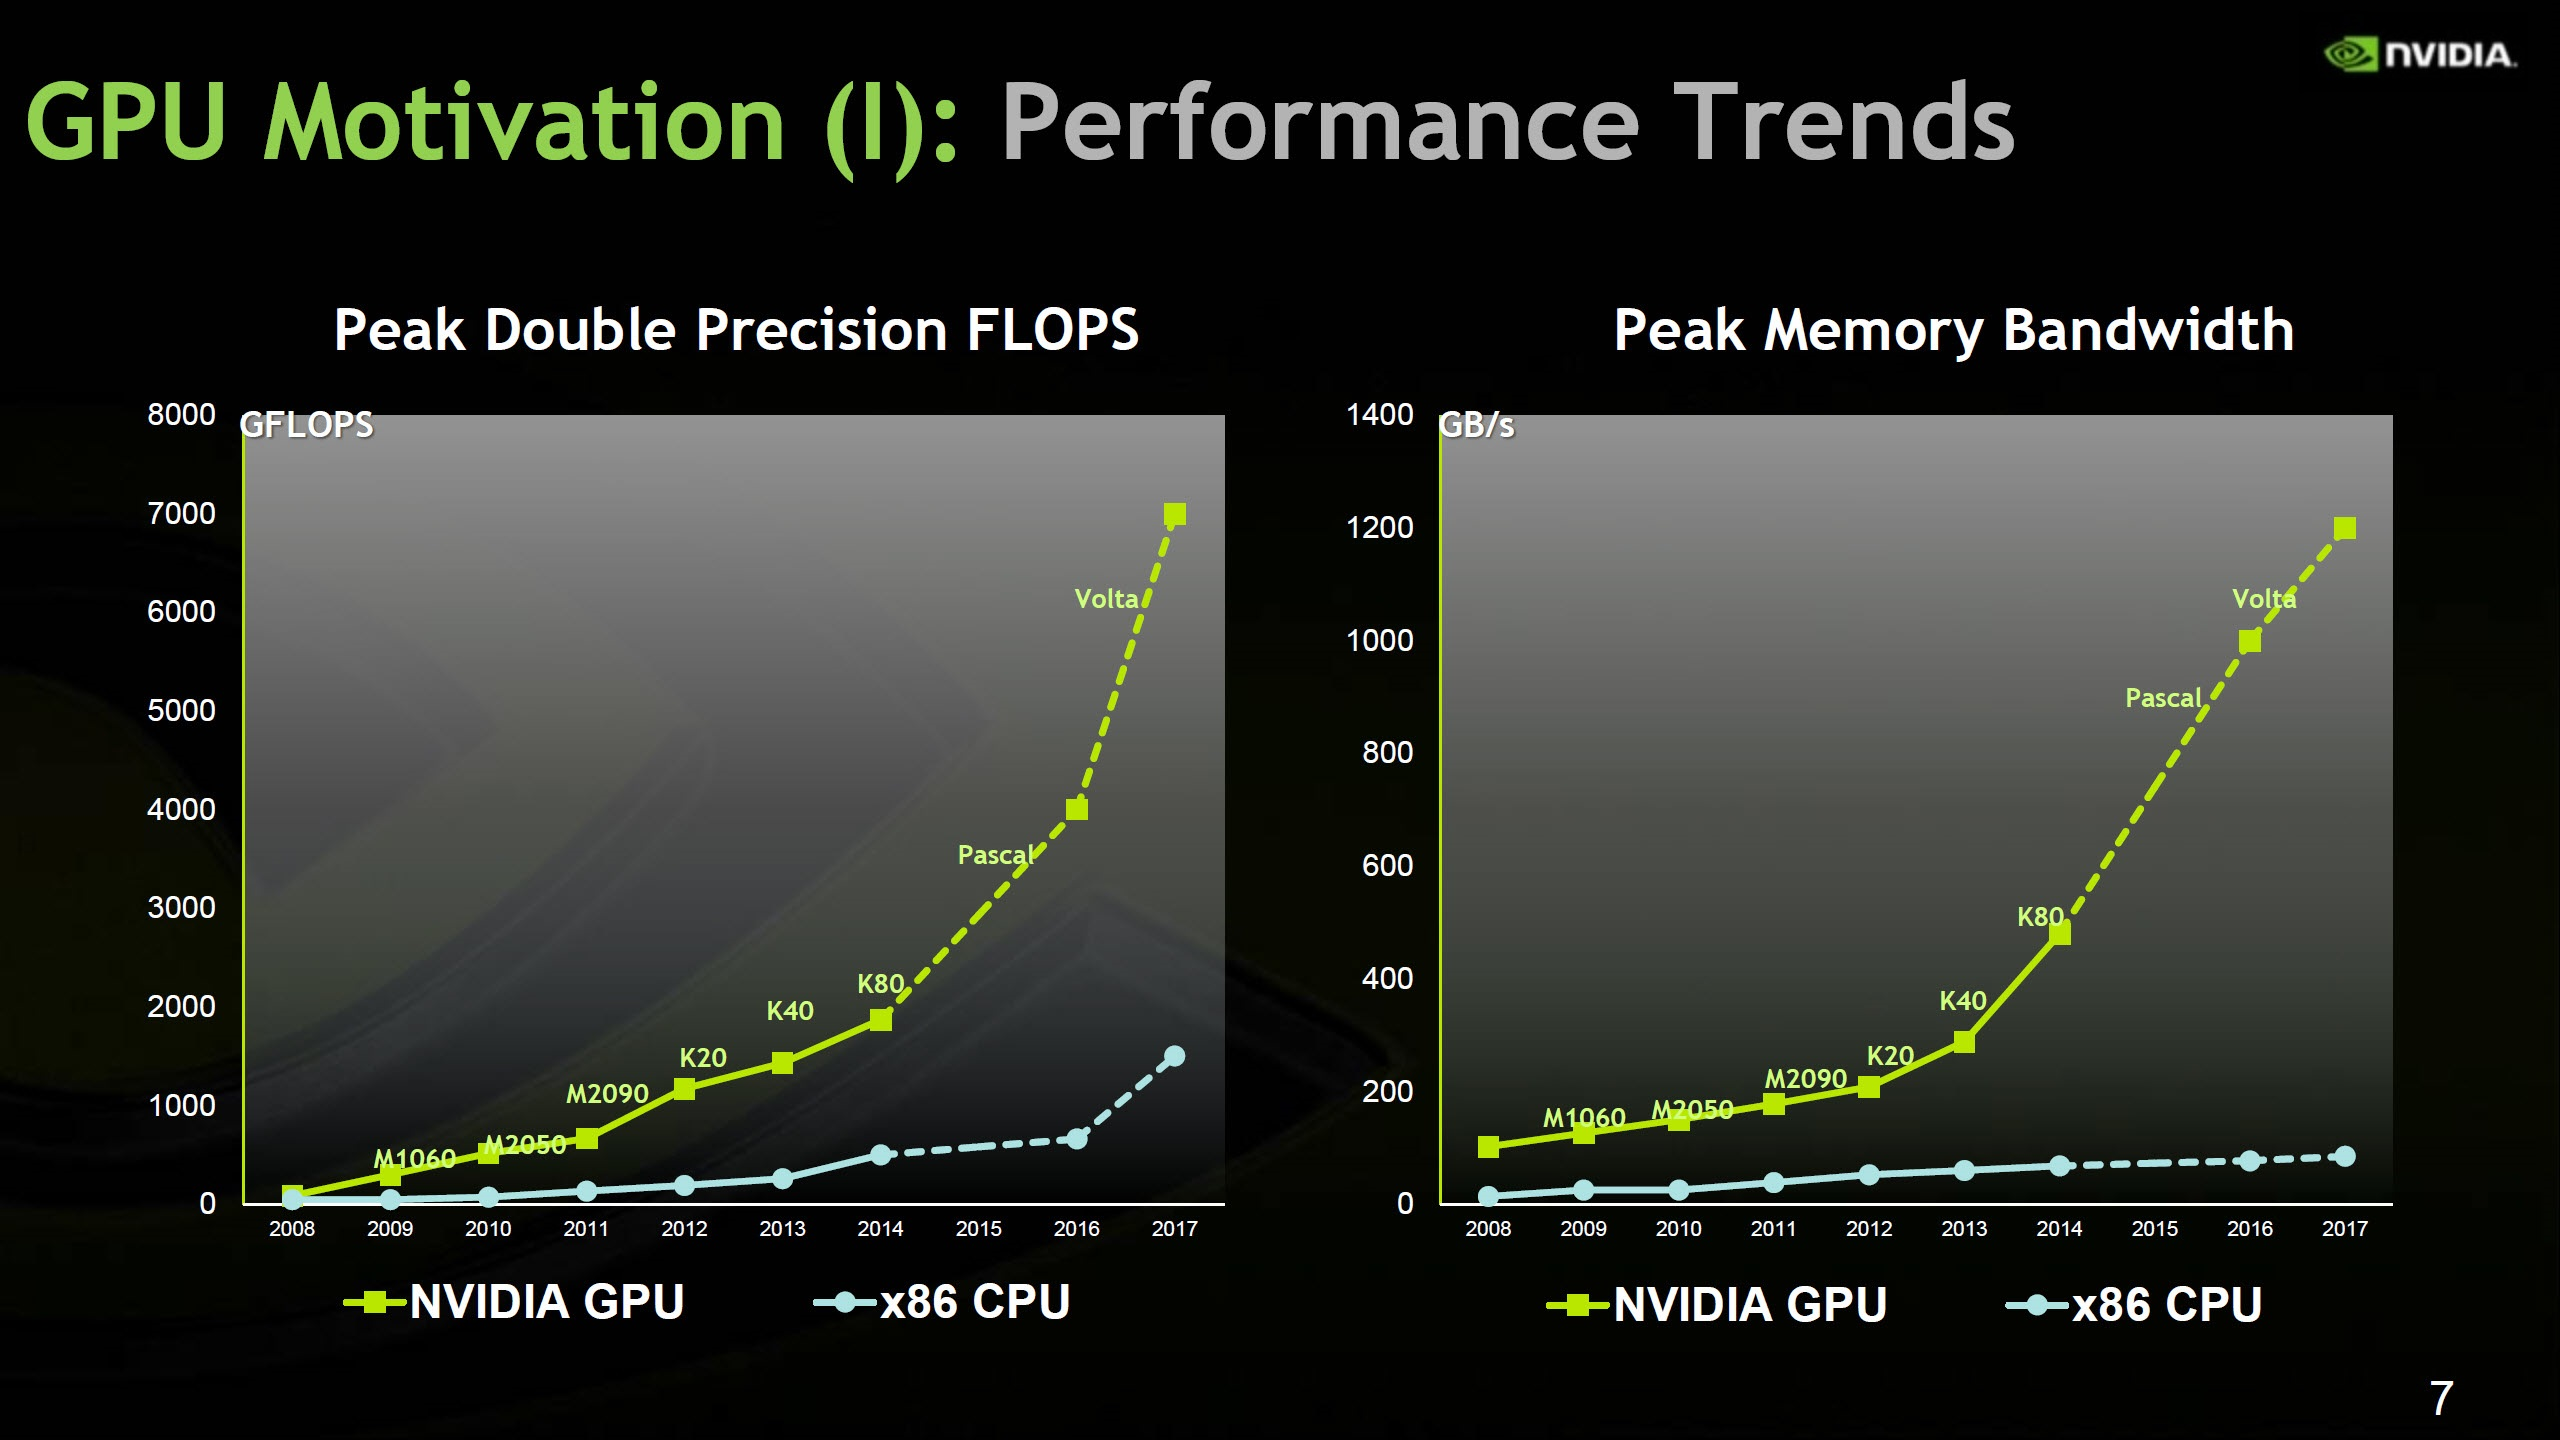
\includegraphics[width=0.85\linewidth]{figures/NVIDIA-Pascal-and-Volta-Compute-Performance.jpg}
    \centering
    \caption{Floating point and bandwidth performance comparison provided by NVIDIA.}
    \label{GPU chart 1}
\end{figure}

\newpage

\section{The MEFD group}

\hspace{5mm}The website of the Department of Mechanical Engineering faculty of the TU/e gives the following description of the MEFD group:\vspace{4mm}

\textit{The MEFD section focuses on the development, analysis and application of mathematical-physical models and advanced numerical techniques for multiscale flow problems in engineering applications, with particular emphasis on flow problems in the transitional molecular/continuum regime and auxiliary field interactions. The research in the section has an underpinning and methodological character, while maintaining a strong connection to applications in the high-tech industry and in other sections.} \autocite[]{tue_mefd_1}\vspace{4mm}

\noindent The work within the MEFD group can be roughly divided into 5 categories:

\begin{itemize}
    \item Research into various models of physics and engineering based problems.
    \item Investigating the mathematical aspects of the aforementioned models.
    \item Evaluating and enhancing discretization techniques and their relation to the models for numerical evaluation.
    \item Implementing the advancements in discretization methods into software (Nutils).
    \item Looking into various algorithms for solving the resulting linear system of equations.
\end{itemize}

The research within the MEFD group into iterative methods, stems from the problems encountered when using the more traditional direct solving techniques in their applications. Methods like LU decomposition can cause excessive run-times or residual errors, making them unsuitable in certain instances. A similar problem can arise when the simulations grow in size. The run-times can grow out of control when the amount of FLOP's required to evaluate the simulations scales badly with the dimensions of the simulation.\vspace{4mm}

The most obvious solution to this problem is to buy computers with increased computational power, but the recent movement towards GPGPU accelerated computers also requires a paradigm shift in programming techniques to leverage their capabilities to the fullest. The MEFD group has recently gained access to a GPGPU enabled server via the Rare Trans project of ASML in conjunction with the Energy Technology group, of which the MEFD group is a part. Its adoption for the simulations of the MEFD group is (at the time of writing) at an early stage.

\newpage

\section{The internship project}

\hspace{5mm}A lot of the numerical methods and simulations that are developed by the MEFD group are based on FEM (or related methods) and often require solving ill-conditioned block-sparse linear systems. These types of applications require relatively large amounts of RAM and double precision floating point data, resulting in additional difficulties when making the transition to GPGPU.\vspace{4mm}

This internship will lay the foundations for a discussion of these difficulties by providing the required background on floating point arithmetic, Amdahl's law and the workings of computers. A high level overview of computers and their history pertaining to scientific computing will be provided, followed by a description of the somewhat more low-level workings of a personal computer. \vspace{4mm}

The final chapter of this report will provide a brief summary of the topics of the master thesis project and their associated challenges.
\chapter{Floating point data}

\hspace{4mm}Floating point data is a common way to store real numbers . Many different types of floating point data types exist, but the most relevant types for scientific computing are:

\begin{itemize}
    \item Double (FP64)
    \item Single (FP32)
    \item Half (FP16)
\end{itemize}

\begin{figure}[h!]
    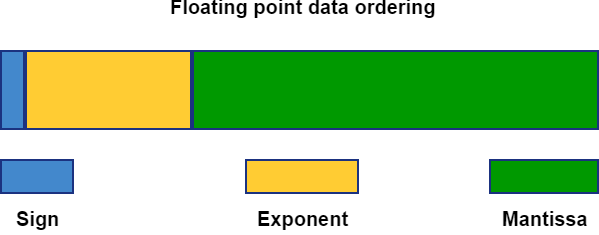
\includegraphics[width=0.6\linewidth]{figures/Float.png}
    \centering
    \caption{Floating point data structure.}
    \label{FP data}
\end{figure}

\vspace{5mm}

Floating point data contains three parts, the sign, the exponent and the mantissa. The sign and exponent are both stored as 2-base little-endian (most significant bit to the left) numbers. The mantissa is treated slightly differently. It is stored as a 2-base big-endian number (most significant bit to the right) with an implicit least significant bit equated to 0.

\subsection*{2-base number conversion}

Equation \ref{example binary eq.} provides an example conversion from the binary representation to the standard 10-base representation.

\begin{equation} \label{example binary eq.}
    \begin{split}
        \text{2 base sign/exponent} & = 0111 \\
        \text{10 base sign/exponent} & =  (8 \times 0) + (4 \times 1) + (2 \times 1) + (1 \times 1) =  7 \\
        \\
        \text{2 base mantissa} & = 0111 \\
        \text{10 base mantissa} & =  (1 \times 0) + (2 \times 0) + (4 \times 1) + (8 \times 1) + (16 \times 1) = 28 
    \end{split}
\end{equation}

\section{Calculating floating point value}

Equation \ref{FP formula eq.} provides the generic conversion formula for FP data. 

\begin{equation} \label{FP formula eq.}
    \text{Value} = -1^{Sign_{2}} \times 2^{Exponent_{10} - Bias_{10}} \times (1 + 1/(Mantissa_{10}))
\end{equation}

\noindent Bias is a data type specific number to "center" the exponent range around 0.

\subsection*{Double (64 bit)}

Common format for sensitive mathematical equations, like solving ill conditioned systems. It is also the default numerical data type of MATLAB.\autocite[]{wiki_double}

\begin{itemize}
    \item Bias: '1023'
    \item Sign: 1 bit
    \item Exponent: 11 bits
    \item Mantissa: 52 bits
    \item Resolution: $ (1/2)^{52} = 2.2204e-16 $
    \item Exponent range: $ 2^{([-1023,1024])} $
\end{itemize}

\subsection*{Single (32 bit)}

Original floating point data type used in 32 bit computers, provides sufficient resolution for many mathematical operations.\autocite[]{wiki_single}

\begin{itemize}
    \item Bias: '127'
    \item Sign: 1 bit
    \item Exponent: 8 bits
    \item Mantissa: 23 bits
    \item Resolution: $ (1/2)^{23} = 1.1921e-07 $
    \item Exponent range: $ 2^{([-127,128])} $
\end{itemize}

\newpage

\subsection*{Half (16 bit)}

Relatively coarse approximation of a real number, but sometimes good enough. A great example of applications that usually don't require more precision are  deep neural networks.\autocite[]{wiki_half}

\begin{itemize}
    \item Bias: '15'
    \item Sign: 1 bit
    \item Exponent: 5 bits
    \item Mantissa: 10 bits
    \item Resolution: $ (1/2)^{10} = 9.7656e-04 $
    \item Exponent range: $ 2^{([-15,16])} $
\end{itemize}

\vspace{5mm}

\newpage
\chapter{Floating point arithmetic}

\section{Fused Multiply Add}

\hspace{4mm}The prolific nature of the dot product in vector mathematics has lead to the development of hardware dedicated to the task, performing a multiplication and addition in a single step:

\begin{equation} \label{FMA eq.}
    \text{A} = \text{A} + \text{B} \times \text{C}
\end{equation}

\noindent It should be noted that the FMA operation can be used to emulate (may take more then a single instruction) the basic operations:

\begin{itemize}
    \item Addition
    \item Subtraction
    \item Multiplication
    \item Division
    \item Raising to a power
\end{itemize}

As such, most modern computers rely on FMA hardware for all their floating point calculations. The low level hardware required to perform the FMA calculation, differs for every floating point format (double, single or half). This makes it a common practice to provide separate hardware blocks for each floating point format.

\newpage
\chapter{Theoretical parallel speedup}

\hspace{4mm} Applying parallel programming techniques to accelerate an algorithm is a very common task. This section will discuss some of the available theory for making predictions about the maximum speedup that can be achieved.

\section{Amdahl's law}

\hspace{4mm} Amdahl's law relates the maximum achievable speedup of a task to the amount of time that the task executes elements that can be parallelized.\autocite[]{wiki_amdahl} This is based on two assumptions:

\begin{itemize}
    \item The task can be divided in a serial part and a parallel part.
    \item The parallel part scales linearly with the amount of available parallel nodes.
\end{itemize}

\begin{equation} \label{Amd 1 eq.}
    \begin{split}
        \text{T}_{total} = & \ \text{T}_{serial} + \text{T}_{parallel}\\
        \text{Speedup}(k) = & \ \frac{\text{T}_{total}}{\text{T}_{serial} + (\frac{\text{T}_{parallel}}{k})}\\
        \\
        k := & \ \text{number of parallel nodes}
    \end{split}
\end{equation}

\vspace{2mm}

As an example, take a task that consist of $95 \%$ parallelizable work. The maximum speedup can never exceed $20$, no matter how much parallel nodes are employed.

\subsection{Parallel slowdown}

\hspace{4mm} Parallel slowdown is an effect that can plague certain parallel tasks.\autocite[]{wiki_parsl} Scaling the task beyond a certain amount of parallel nodes causes a runtime increase instead of the expected decrease. This is typically associated with a communications bottleneck, where the time required for communication between the parallelly executed parts grows faster than can be compensated by dividing the workload among the parallel nodes.

\newpage

\section{Compensated Amdahl's law}

\hspace{4mm}Amdahl's law assumes that dividing the parallel part of the task among many nodes doesn't inflict any sort of runtime penalty. That assumption is certainly reasonable for embarrassingly parallel workloads, but is not always correct outside of the embarrassingly parallel case.\\

\noindent Amdahl's law can be compensated for this runtime penalty by specifying and additional part of the task, called $\text{T}_{overhead}(k)$, which is modelled as a function of the amount of nodes:

\begin{equation} \label{Amd 2 eq.}
    \begin{split}
        \text{T}_{total} = & \ \text{T}_{serial} + \text{T}_{parallel}\\
        \text{Speedup}(k) = & \ \frac{\text{T}_{total}}{\text{T}_{serial} + (\frac{\text{T}_{parallel}}{k}) + \text{T}_{overhead}(k)}\\
        \\
        k := & \ \text{number of parallel nodes}
    \end{split}
\end{equation}

\vspace{2mm}

\noindent The exact relation between $\text{T}_{overhead}(k)$ and the amount of nodes is application specific, but two general modelling assumptions seem reasonable:

\begin{itemize}
    \item There is no overhead when only one node is available.
    \item $\text{T}_{overhead}(k)$ consists of a parallelizable and non-parallelizable part.
\end{itemize}

The first assumption is trivial. The second one states that the tasks constituting the overhead can consist of elements that need to be executed sequentially and elements that can be executed concurrently.

\subsection{Modelling parallel slowdown}

\hspace{4mm} Parallel slowdown can be modelled with the compensated Amdahl's law. When it is indeed caused by a communications bottleneck, it seems reasonable to assume the following things:

\begin{itemize}
    \item The overhead consists exclusively of non-parallelizable tasks.
    \item The overhead scales linearly with the amount of parallel nodes.
\end{itemize}

Communication between multiple nodes is usually dominated by non-parallelizable tasks, because it often involves some form of causality. The choice of scaling is debatable, but less then linear scaling is very unlikely, whereas more than linear scaling is very common.\\

\noindent The predicted speedup would in this case be:

\begin{equation} \label{Amd 3 eq.}
    \begin{split}
        \text{T}_{total} = & \ \text{T}_{serial} + \text{T}_{parallel}\\
        \text{Speedup}(k) = & \ \frac{\text{T}_{total}}{\text{T}_{serial} + (\frac{\text{T}_{parallel}}{k}) + ((k - 1) \times \text{T}_{overhead})}\\
        \\
        k := & \ \text{number of parallel nodes}
    \end{split}
\end{equation}

\newpage

\subsection{Compensated example}

\hspace{4mm} An example will be discussed to illustrate the consequences that the overhead compensation of Amdahl's law can have. Like the previous example, the parallel part of the task is set at $95 \%$. The relation for $\text{T}_{overhead}(k)$ is taken from the communications bottlenecked case, with a constant factor of $1 \%$ of $\text{T}_{total}$.

\begin{figure}[h!]
    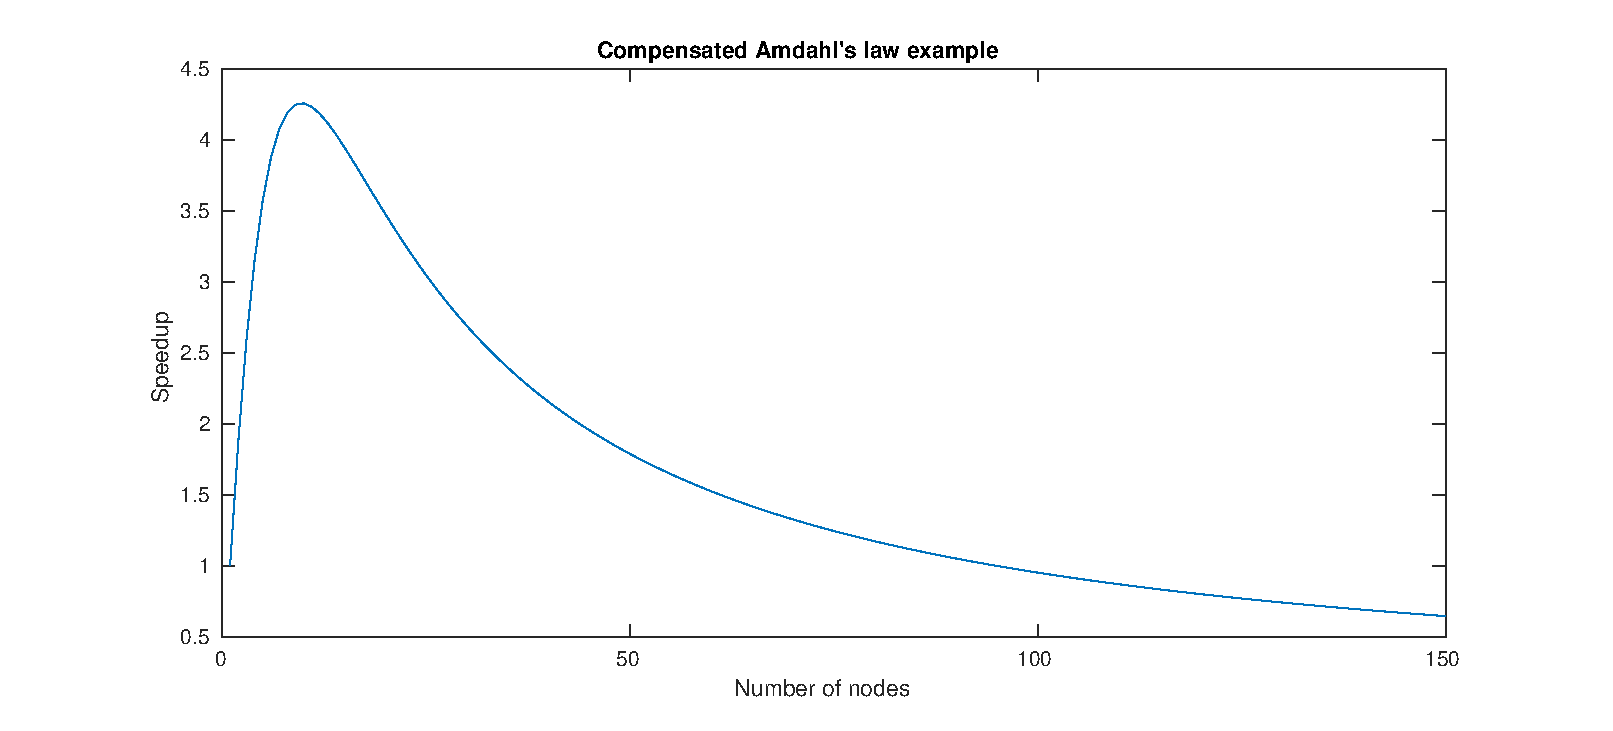
\includegraphics[width=\linewidth]{figures/Compensated_amdahl.eps}
    \centering
    \caption{Task: $95 \%$ parallelizable, $5 \%$ serial and $1 \%$ overhead.}
    \label{com. amd. ex.}
\end{figure}

The maximum speedup of about $4.255$ is achieved using $10$ parallel nodes, a far cry from the maximum of $20$ that the uncompensated Amdahl's law predicted. Using $150$ nodes results in a speedup of about $0.65$, which is actually a significant performance decrease.

\newpage

\section{Experimental verification}

\hspace{4mm} Accelerating iterative solvers by dividing the workload among parallel nodes is a common practice. However, there is a general rule of thumb that the amount of parallel nodes should not be to large in these cases, as the communication between the processes quickly becomes excessive.\\

\citeauthor{dist_it_solv} investigated the scaling behaviour of distributed iterative solvers, focusing on the Gauss-Seidel method\autocite[]{dist_it_solv}. They provide experimental data on the scaling behaviour for three kind of sparsity patterns:

\begin{figure}[h!]
    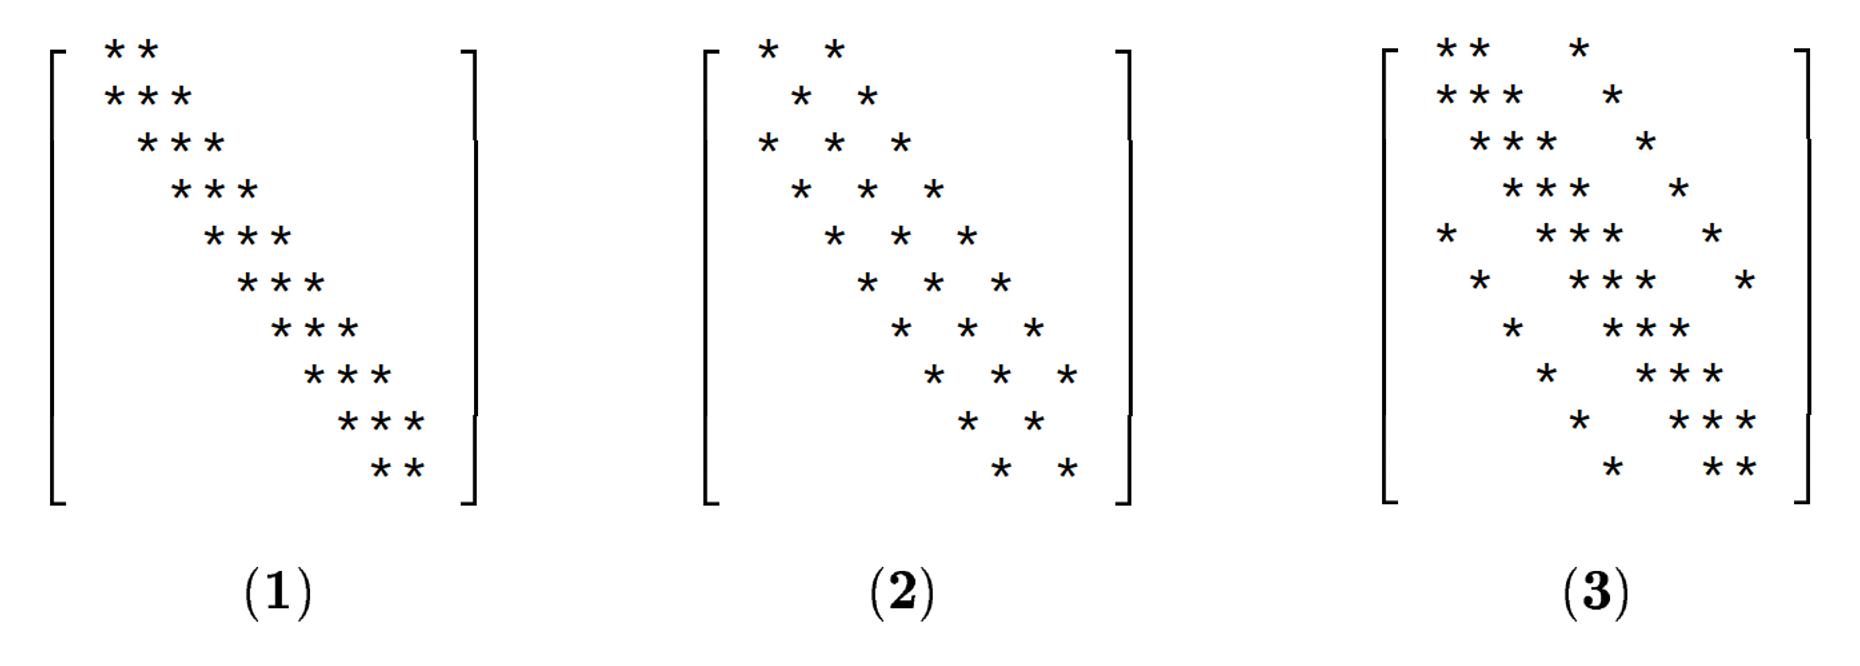
\includegraphics[width=0.6\linewidth]{figures/Amd_sparse.png}
    \centering
    \caption{Density: $(1) = 0.015$, $(2) = 0.015$, $(3) = 0.025$ \\ (Taken from \citeauthor{dist_it_solv})}
    \label{com. amd. sp.}
\end{figure}

\begin{figure}[h!]
    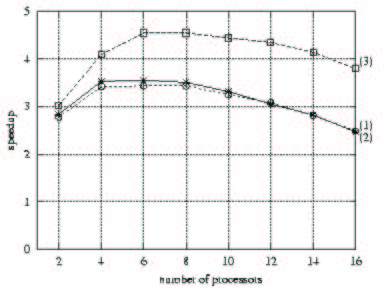
\includegraphics[width=0.5\linewidth]{figures/Amd_scale.png}
    \centering
    \caption{Speedups of distributed iterative solvers.\\ (Taken from \citeauthor{dist_it_solv})}
    \label{com. amd. sc.}
\end{figure}

\noindent Figure \ref{com. amd. sc.} shows three things:

\begin{itemize}
    \item Parallel slowdown occurs for all three matrices when using more then $8$ processors.
    \item Sparsity pattern has little effect on the speedup.
    \item Density has a significant effect on the speedup.
\end{itemize}

Worth mentioning is the questionable speedup at $2$ processors, having a value of about $3$ for all three curves. This is odd because Amdahl's law states that the speedup can never exceed the amount of parallel nodes. It might be explained by some caching effect, where the complete data set doesn't fit in the cache of a single processor, but does fit in the cache of two processors. No mention of this was made by \citeauthor{dist_it_solv}.\\

\subsection{Fitted model results}

\hspace{4mm} To evaluate the performance of the compensated Amdahl's law, a comparison is made with the experimental data of \citeauthor{dist_it_solv}.\\

The model represented by equation \ref{Amd 3 eq.} was selected for the comparison, because it is expected that the parallel slowdown was caused by a communications bottleneck. $\text{T}_{parallel}$ was set to $100 \%$ because the algorithm used by \citeauthor{dist_it_solv} contains no serial part. Some experimenting provided the values of $\text{T}_{overhead}$:

\begin{figure}[h!]
    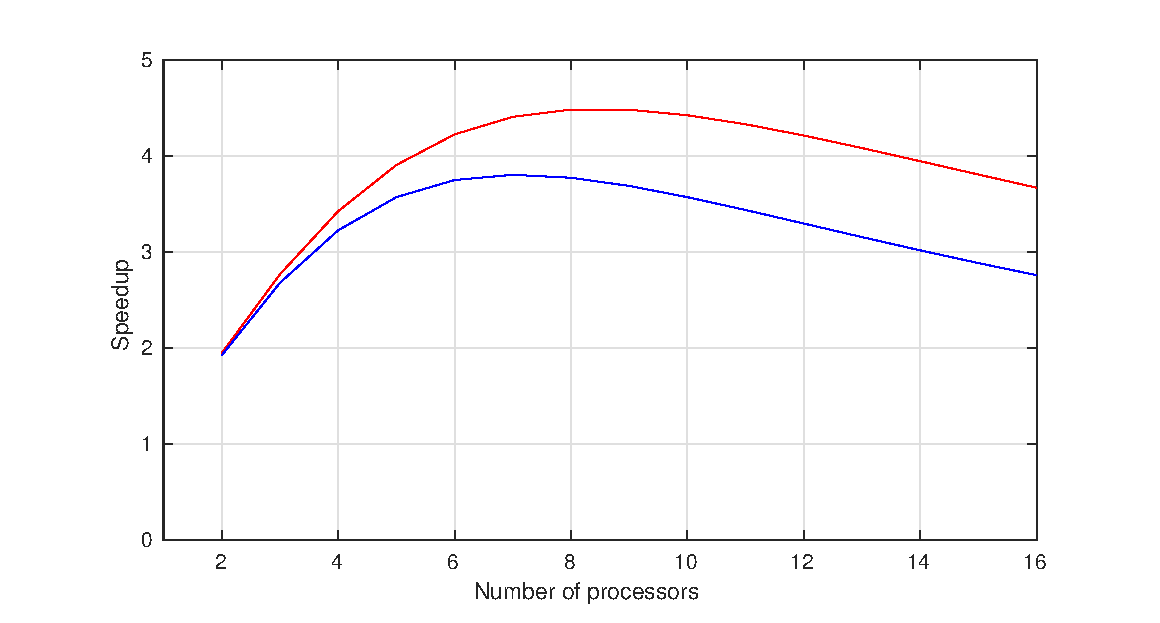
\includegraphics[width=0.7\linewidth]{figures/Amd_ver.eps}
    \centering
    \caption{Red: $\text{T}_{parallel} = 100 \%$, $\text{T}_{overhead} = 1.4 \%$\\
    Blue: $\text{T}_{parallel} = 100 \%$, $\text{T}_{overhead} = 2.0 \%$}
    \label{com. amd. ver.}
\end{figure}

The results are not too bad. The behaviour in the region between $2$ and $6$ processors is a little different, but speedups exceeding the number of parallel nodes cannot be explained with Amdahl's law. Some unknown effect must have had a significant influence on the results of the experimental data, but it is generally very uncommon to see this kind of behaviour.\\

The value of the maximum speedup and the amount of processors required to achieve said speedup are relatively accurate. The experimental results show a slightly less linear and steeper descend then the model, but this just means that the assumption that the overhead scales linearly with the amount of parallel nodes is not completely true. This reflects the discussion of the model provided at section "Modelling parallel slowdown".\\

The red line models the situation of matrix $(3)$, with a density of $0.025$. The blue line models the two other cases with the lower density of $0.015$. The higher density situation has a lower overhead, $1.4 \%$ versus $2.0 \%$. This appears reasonable, because the higher density results in a higher runtime per processor, while the communication overhead remains unaffected. As $\text{T}_{overhead}$ is modelled as a fraction of $\text{T}_{total}$, this lower $\text{T}_{overhead}$ is to be expected.
\chapter{Computer models}

\section{Personal computer model}

\hspace{4mm}The traditional personal computer was designed to perform many different operations on a relatively small amount of data. Because parallelising many different operations on the same data is very hard to impossible, sequential execution of the operations has long been (still is) the norm. The result is a combination of a few very fast execution units in the CPU and a "pyramid shaped" memory/storage system. 

\begin{figure}[h!]
    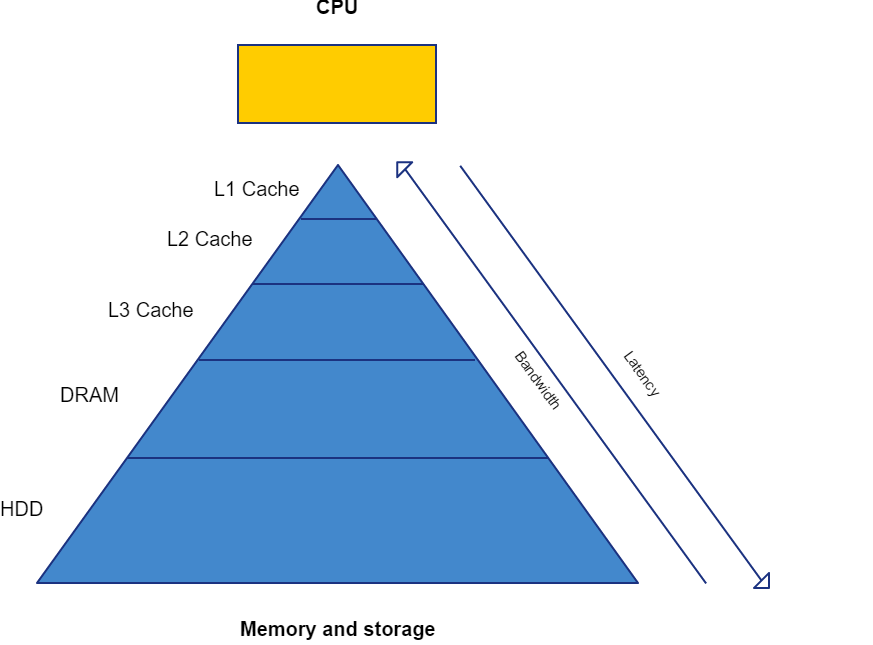
\includegraphics[width=0.65\linewidth]{figures/Traditional-computer.png}
    \centering
    \caption{Abstract representation of the traditional personal computer.}
    \label{Piramid}
\end{figure}

\subsection*{Pyramid shape}

\hspace{4mm}Creating fast memory is expensive and not all the available data needs to be instantly accessible. Production cost savings led to a small amount of very fast memory close to the execution units, called "Cache". A larger amount of significantly slower memory, called "RAM", acts as the data overflow buffer of the cache. The lowest layer of memory consists of non-volatile storage, often in the form of an HDD or SSD, which contains the data that the needs to survive a power cycle.\vspace{5mm}

As CPU's grew more capable, and the way in which they where used, changed over the years, additional layers (L2 and L3) of cache where added to accommodate.

\section{Bandwidth}

\hspace{4mm}Bandwidth is one of two measures of the "speed" of memory, but bandwidth is a broader concept. Bandwidth is a measure of the maximum amount of data that can be transferred between a sender and a receiver within a time-frame\autocite[]{wiki_bandwidth}. Data transfer channels are usually bi-directional, making the distinction between sender and receiver less relevant.\vspace{5mm}

High data transfer rates are desirable, but like storage capacity, are costly to achieve. The traditional computer model benefits most from high memory bandwidth at the cache level and becomes less important towards the bottom of the "pyramid".\vspace{5mm}

The most common measure for bandwidth is bytes per second, a table of derived units and their meaning is provided by table \ref{bandwidth table}. A bit is a single one or zero and a byte is a set of 8 bits.

\begin{table}[h!]
    \centering
    \caption*{\textbf{Bandwidth}}
    \begin{tabular}{l c c c || r r r r} 
        \hline
        kilo & mega & giga & terra & & & & bits per second \\ 
        \hline\hline
        Kb/s & Mb/s & Gb/s & Tb/s & 1.000 & 1.000.000 & 1.000.000.000 & 1.000.000.000.000 \\ 
        KB/s & MB/s & GB/s & TB/s & 8.000 & 8.000.000 & 8.000.000.000 & 8.000.000.000.000 \\
        Kib/s & Mib/s & Gib/s & Tib/s & 1.024 & 1.048.576 & 1.073.741.824 & 1.099.511.627.776 \\
        KiB/s & MiB/s & GiB/s & TiB/s & 8.192 & 8.388.608 & 8.589.934.592 & 8.796.093.022.208\\
        \hline
    \end{tabular}
    \caption{Acronyms to the left and their numerical values to the right.}
    \label{bandwidth table}
\end{table}

\section{Latency}

\hspace{4mm}Memory latency is a highly multifaceted topic, which is largely beyond the scope of this text, but should be understood at a global level to appreciate the performance impact on certain algorithms. Latency, or access time, is defined as the amount of time between a request to a system and the response of the system.\autocite[]{wiki_latency} Memory latency is the second important measure of the "speed" of memory.\vspace{5mm}

In order to understand memory access time, one must first (roughly) understand how memory is accessed. Computer memory is a highly structured and complex system, with many different layers and subsystems (cache, RAM, HDD). The steps that are required to access data from computer memory are dictated by the structure of the global computer memory system, but also by the local structure of the memory subsystem that contains the data. These local structures can vary pretty significantly from subsystem to subsystem, but they all "group" their resources into "memory blocks", which contain the actual data. The nature of these "blocks" is defended by the precise structure of the specific memory subsystem.\vspace{5mm}

When the user makes a request to access certain (parts) of data, a list of "storage addresses" is generated. This list of "storage addresses" maps to the memory subsystem and corresponding memory blocks that contain the requested data. This list of storage addresses is passed through to the relevant memory subsystem and then gets processed. This results in the data contained in the memory blocks being presented to one or more of the outputs of the memory subsystem in a serial fashion.\vspace{5mm}

\newpage

The time between the arrival of the storage addresses list and the moment the first block of data is presented, is called latency of that memory subsystem. The total latency of a data access request is the amount of time from the moment a "gather" instruction is issued till the moment that the data is "gathered" (available for manipulation).\vspace{5mm}

Latency is usually measured in mili/nano seconds, but can also be provided in cycles. This is equivalent to time, because each cycle takes a set amount of time (dependant on operating frequency).

\section{Scientific computing}

\hspace{4mm}The traditional personal computer model is optimized to perform many different operations on a small amount of data, but most workloads of a scientific computing nature are characterized by many similar operations on a large amount of data. Take for example a matrix-matrix multiplication, which consists of many floating point multiplications and additions, operating on two large amounts of data. This difference doesn't exclude scientific computing related tasks from running on personal computers, but the (personal computer) hardware is not tailored towards the task, resulting in performance that leaves a lot to be desired.\vspace{5mm}

As the personal computer became faster, consumers where interested in using their computer for more than just office related workloads. Content creation like photo and video editing, but also gaming, are prime examples of these more modern tasks for the personal computer. These tasks are like scientific computing tasks, in the sense that they involve floating point operations on large data sets. This resulted in the development of much more powerful graphics cards, specifically for applications that required manipulations on graphical data sets, like decoding (viewing) video files or playing video games.\vspace{5mm}

Meanwhile, scientific applications did not really see the development of specialized hardware. The only way to scale the performance of these tasks was to divide the workload among many computers organized in "clusters", relying on hardware that was developed mostly for hosting large relational databases. Database related workloads require fast non-volatile storage and the ability to handle many different requests. These requirements are similar to those of scientific computing, but are still very different in key aspects. Firstly, a request to a relational database does not require floating point operations. Second, the scale of relational databases often approach the terabyte range, making the capacity of RAM woefully insufficient. Typical medium to large scale scientific computing workloads don't exceed more than a couple of gigabyte of data, and as such are best stored in RAM.\vspace{5mm}

The big game changing moment for scientific computing came when certain scientists realized that graphics cards, developed for consumers, could be very suitable for the needs of scientific computing. The only real problem was that the applications had to be programmed using graphics API's, like DirectX, making the process of writing simulations very difficult and restrictive. One of the main producers of graphics cards, NVIDIA, saw this problem and decided to alleviate some of these difficulties by making (relatively) slight modifications to graphics cards. The result, CUDA cores and CUDA toolkit, allowed for much easier and less restricted access to the resources provided by graphics cards for scientific computing workloads.

\newpage

\section{Personal vs Massively Parallel computer model}

\hspace{4mm}The Massively Parallel computer model differs from the traditional personal computer model in many ways because it focuses on simultaneous execution of computations\autocite[]{wiki_mp}. To understand why parallel execution is fundamental for scientific computing, a very low level problem called the "power wall" should be explained.\vspace{5mm}

CPU's and GPU's are made from transistors, which can be switched "on" or "off". A transistor is on when electrical current can flow through it, making it conductive. A transistor is off when electrical current cannot flow through it, making it non-conductive (hence the term semiconductors). Switching the state of a transistor requires a small amount of electrical current, the energy of that current needs to be dissipated in the form of heat. When a transistor is required to switch ever faster, because the performance of a CPU (or GPU) scales linearly with it's operating frequency, the current required to switch the state of the transistor also increases. The kicker is that the amount of current required to switch the state of a transistor scales quadratically with the switching frequency (caused by parasitic capacitance at the transistor). The final result is that attempts to increase the performance of a CPU or GPU by increasing its operating frequency are frustrated by a quadratic increase in power consumption and heat production, which at some point makes increasing the operating frequency impossible. This limit is called the "power wall".\vspace{5mm}

Scaling the performance of a CPU or GPU by increasing the amount of execution units or cores has no such problems, but faces other difficulties, the biggest of which is causality. When the result of problem X is (deterministically) dependent on the result of problem Y, it follows that problem Y should be solved before problem X can be solved. These types of situations are extremely difficult (or impossible) to accelerate with parallel execution.\vspace{5mm}

Many scientific computing workloads, like the aforementioned example of matrix-matrix multiplication, are known to be "embarrassingly parallel"\autocite[]{wiki_embarrassing}. This means that parallel execution isn't hindered by causality related problems and as such yields the greatest performance (per Watt) on massively parallel systems, like GPU's.
\chapter{Central processing unit}

\section{Basics of a CPU}

\hspace{4mm}Processors, or CPU's, are the "beating heart" of a computer, and as such, perform many more tasks than the ones that will be discussed in this text. The focus lies on the floating point calculation capabilities and the memory subsystems, as well as the interfaces.\vspace{5mm}

The traditional CPU\autocite[]{wiki_cpu} is an integrated circuit that executes the logic, arithmetic , input/output (I/O) and control operations that are prescribed by software running on the computer. As time passed, many other subsystems of computers got integrated into the processor package (die), making the functions that the traditional CPU performs only a subset of all the functions that a modern processor performs. A "core" of a modern processor is a separate unit that performs all the tasks of a traditional CPU.\vspace{5mm}

Modern processor cores are very diverse, complex and multi-faceted, varying wildly with ISA, microarchitecture, intended platform and manufacturer. A discussion about CPU's that would include all these variations would be impossible, necessitating a confinement. This discussion will try to be as generic as possible, but the focus lies on an Intel based server CPU of the "Skylake-SP" microarchitecture.\vspace{5mm}

Intel dominates the PC/laptop as well as the HPC/Supercomputer CPU market, making the restriction towards an Intel x86-64 based CPU justified. Considering the fact that almost all Laptops and workstations contain CPU's that are (to a varying extend) derived from their server oriented counterparts, focusing the discussion around a server CPU seems logical as well. The Skylake-SP microarchitecture was chosen because it is very recent (at the time of writing), contains some very significant advancements for scientific computing workloads and is used in a cluster available to the MEFD group at the TU/e.

\newpage

\section{System on a Chip}

\hspace{4mm}Modern processors are best described by the "System on a Chip"\autocite[]{wiki_cpu} moniker, containing many of the core components of a computer. As such, most contain the following subsystems:

\begin{itemize}
    \item Cores
    \item Memory controller
    \item Cache
    \item Interfaces
    \item Graphics (included in most consumer oriented CPU's)
\end{itemize}

\section{Instruction set architecture}

\hspace{4mm}An Instruction Set Architecture is an abstract model of a computer and contains a collection of machine instruction definitions\autocite[]{wiki_isa}. Examples of common ISA's are x86-64, x86 and ARM, with x86-64 being the most common ISA for CPU's in servers, as well as consumer oriented computers.\vspace{5mm}

An ISA is one of the most important aspects of a CPU, because it forms the link between software and hardware. ISA's where introduced to make programming software easier, which could now be written in terms of ISA instructions in stead of low level machine code\autocite[]{wiki_mc}. This made it possible to execute the same computer program on different computers, without any modification of the code.\vspace{5mm}

An implementation of an ISA, called a microarchitecture (uarch)\autocite[]{wiki_ua}, is the hardware based realization of these machine instruction definitions (disregarding microcode\autocite[]{wiki_uc}). Any specific uarch can also support extensions to its ISA, common examples are VT-d, AES-NI, SSE4 and AVX2. These extensions are additions to the abstract computer model of an ISA and contain specific instructions to accelerate certain tasks of a computer, like AES data encryption, virtualization and vector mathematics.\vspace{5mm}

Some better known examples of microarchitectures are Intel i386, Intel Nahelem, Intel Haswell, AMD K8, AMD Bulldozer and AMD Zen. 

\newpage

\section{Threads and cores}

\hspace{4mm}A thread is a chain of instructions that is to be executed by the CPU\autocite[]{wiki_thread}. Each thread is generated by a process, which can loosely be described as an instance of a computer program. A single core of a CPU can execute one thread at a time, but using a technique called time slicing and the concept of context switching\autocite[]{wiki_cs}, can handle multiple threads concurrently.\vspace{5mm}

Multithreading (software) allows a single process to spawn a multitude of threads, dividing the workload of that process. Performance benefits (can) arise when these threads are executed in parallel on multiple cores of a CPU.\vspace{5mm}

The specifications of a CPU may contain references to the number of threads it "has", which should be interpreted as the maximum amount of threads it can "execute" at the same time. The fact that a single CPU core can only execute one thread at a time doesn't change, even if the CPU specifications state that it has more (twice) threads then cores. This has to do with a hardware based technique called simultaneous multithreading\autocite[]{wiki_smt}, which will be discussed later.

\section{Cache}

\hspace{4mm}Quick access to data is critical for the performance of a CPU, making data flow and storage a mayor aspect of a CPU. The main memory of a computer has a relatively high latency and low bandwidth compared to the needs of modern CPU cores, which is where cache comes into play\autocite[]{wiki_cache}.\vspace{5mm}

Cache is storage subsystem of the CPU and acts like a data buffer. It contains, among other things, copies of the data that the CPU (or process) "predicts" it will access often or in the near future, reducing the loading time of that data. The amount of cache placed on the CPU is relatively small, typically about 1:1.000, compared to the amount of main memory placed in a computer. A "cache-miss" refers to the situation where data is requested, but not stored in cache, resulting in a much longer loading time. Avoiding cache-misses is a large part of software (and hardware) optimization and can lead to very substantial performance improvements.\vspace{5mm}

Cache memory pressure (memory nearly full) and the ever increasing speed of CPU cores lead to the development of multiple levels of cache. This layered structure has the advantage that it can address both the memory pressure problem as well as the demand for faster data access, without resulting in prohibitive costs. The upper most layer of cache, L1, has gotten significantly faster over time, but did not really increase much in capacity. The lowest level of cache, typically L3, saw the highest increase in capacity, but is also substantially slower then L1.\vspace{5mm}

The development of multi-core processors and several levels of cache created an additional task for cache; inter-core data communication. Each core has its own private parts of L1 and L2 cache, whereas L3 cache is shared between the cores. This last level of cache is the place where data can be shared between the threads running on the different cores.\vspace{5mm}

\newpage

Cache memory is a lot faster, and generally superior on many fronts, compared to main memory, because cache is made from SRAM and main memory is made from DRAM. SRAM stands for "Static Random Access Memory", whereas DRAM stands for "Dynamic Random Access Memory". Each SRAM memory cell requires 6 transistors to store a bit, whereas DRAM requires only one transistor (and a small capacitor) per bit. The downside of DRAM is that the capacitors in DRAM memory need to be recharged frequently, causing delays and other problems. This constant refreshing of the stored data gave rise to the name "Dynamic", while "Static" was used for SRAM, because it doesn't need to be refreshed. The extra hardware complexity of SRAM allows it to be much faster than DRAM, but the extra cost and space requirements on the die of the CPU also make it much more expensive.

\section{Execution units}

\hspace{4mm}Execution units of a CPU core are the parts that execute the machine instructions derived from the thread running on the core. There are many different types of execution units in modern CPU cores, each with their own specific function. Notable examples of execution units are; arithmetic logic unit\autocite[]{wiki_alu}, address generation unit\autocite[]{wiki_agu} and floating-point unit\autocite[]{wiki_fpu}. Discussing the functions and operations of all these execution units is beyond the scope of this text, which will focus on the floating-point execution unit.

\subsection*{Superscalar}

\hspace{4mm}CPU cores have many execution units, most also have multiple execution units of the same type. Keeping all the execution units busy at the same time requires multiple instructions to be dispatched (one instruction per execution unit) simultaneously. The ability of a CPU core to dispatch multiple instructions simultaneously is called being superscalar\autocite[]{wiki_super}, whereas CPU's that can only dispatch a single instruction are called scalar. Superscalar capabilities are a form of instruction-level parallelism\autocite[]{wiki_ilp}.

\subsection*{SIMD}

\hspace{4mm}SIMD\autocite[]{wiki_simd} stands for single instruction, multiple data and is a form of data level parallelism\autocite[]{wiki_dlp}. SIMD is a vector processing technique, allowing an execution unit to perform the same instruction on multiple data entries (grouped in 1D arrays called vectors) in a single clock cycle. The maximum achievable throughput increases substantially by using SIMD, but does requires all the data to be manipulated in the same way, making it less versatile.\vspace{5mm}

SIMD works by exposing deep registers to execution units, containing the data vectors\autocite[]{wiki_register}. The instruction that the execution unit receives is performed on the complete register.

\newpage

\subsection*{FMA3 and advanced vector extensions}

\hspace{4mm}The floating-point execution units found in modern Intel CPU cores are based on FMA3 (from Haswell on wards). These FMA based units are capable of three different operations:

\begin{itemize}
    \item $ a = a \cdot c + b $
    \item $ a = b \cdot a + c $
    \item $ a = b \cdot c + a $
\end{itemize}

The Skylake-SP uarch contains two AVX-512 execution units, with 512 bit deep registers. Each AVX-512 unit contains 8 FMA3 sub-units for "double" floating-point numbers and 16 FMA3 sub-units for "single" floating-point numbers. These AVX-512 execution units form the hardware layer of the AVX-512 ISA extension\autocite[]{wiki_avx512}.\vspace{5mm}

The Haswell and Broadwell uarch contain two AVX2 execution units, with 256 bit deep registers. Each AVX2 unit contains 4 FMA3 sub-units for "double" floating-point numbers and 8 FMA3 sub-units for "single" floating-point numbers. These AVX2 execution units form the hardware layer of the AVX2 ISA extension\autocite[]{wiki_avx2}.\vspace{5mm}

AMD's latest (at the time of writing) Zen architecture also supports AVX2 instructions (not AVX-512), but the hardware based implementation is completely different. It doesn't have native support for 256 bit deep registers and each AVX2 instruction takes 2 clock cycles to complete, compared to one clock cycle of Intel based AVX2 capable CPU's.

\section{Simultaneous multithreading}

\hspace{4mm}Simultaneous multithreading, also known as Hyper-Threading\autocite[]{wiki_ht}, is a technique aimed at increasing the utilization of a CPU core. Each physical CPU core represents multiple logical CPU cores, fully transparent to the Operating System. Every logical CPU core gets their own thread assignment by the OS, meaning that a single CPU core is tasked with multiple threads. The amount of logical cores per physical core differs from microarchitecture to microarchitecture. The most common is two logical cores per physical core, but Intel Xeon Phi\autocite[]{wiki_phi} and IBM POWER9\autocite[]{wiki_p9} based designs have 4 and up to 8 logical cores per physical core.\vspace{5mm}

When a thread (assigned to a CPU core) is unable to assign tasks to every execution unit of the CPU core, instructions of a different thread assigned to the same CPU core can be dispatched to the unused execution units. One of the most common culprits for a thread to under utilize the execution units, is cache misses. SMT can be very helpful in hiding the latency caused by data requests that require multiple clock cycles to fulfill.\vspace{5mm}

The performance improvements generated by SMT vary wildly with applications, from a factor of two down too a performance decrease. SMT has the largest positive effect in situations where cache-misses are frequent, instruction level parallelism per thread is low and the workloads of the threads are very heterogeneous. Math routines provided by highly optimized libraries, such as the Intel Math Kernel Library\autocite[]{wiki_mkl}, generally don't fall into this category, making SMT less beneficial for HPC purposes.\vspace{5mm}

\newpage

\section{Operating frequency}

\hspace{4mm}The (high level) building blocks of digital circuits are called logic gates, which are hardware implementations of boolean operations. These logic gates are combined in intricate ways to provide more high level functionality, like the FMA operation on floating-point data. Synchronization of the logic gates is key for their operation, which is where the clock signal comes into play\autocite[]{wiki_clock}.\vspace{5mm}

The clock signal of the CPU core is a square wave signal, switching between high and low (logical "on" and "off"). The rising and falling edges of this square wave are the "timing" signals for the logic gates to evaluate their input. The frequency of this timing signal is called the operating frequency or clock frequency of the CPU core. The operating frequency of a CPU core is directly linked to the throughput of micro-operations\autocite[]{wiki_uop}, making it a key factor in the performance of a CPU.

\subsection*{Turbo frequencies}

\hspace{4mm}Almost all modern CPU's employ some sort of dynamic operating frequency control, allowing the operating frequency of various parts of the CPU to go up or down in conjunction with demand and thermal headroom. Dynamic scaling of the operating frequencies took a flight when mobile devices became more popular, requiring momentary high performance and long battery life. The basic idea behind these techniques is that a relatively high operating frequency can be achieved for a short duration of time. This increases performance for workloads that can be completed within the time frame of the elevated operating frequency, but doesn't significantly increase the overall heat production and power consumption of the CPU. The turbo boost technology of modern CPU's is too complex to discuss in great detail in this text, but a few important aspects pertaining to floating point performance will be explained.\vspace{5mm}

Specifications of the turbo frequencies are very important to the performance of a CPU, but are often reduced to a single number, masking the complete story for marketing purposes. Turbo frequencies scale down according to the workload type (normal, AVX2 and AVX512) and the amount of active cores. AVX512 workloads produce the most heat and highest power consumption because their execution units contain the most transistors, AVX2 execution units require less power and normal (non floating-point) workloads even less than that.\vspace{5mm} 

A more detailed specification of the turbo frequencies of an Intel Xeon Gold 6132 CPU will be provided as an example. Intel ark based information on the Xeon Gold 6132 specifies a base frequency of 2.6 GHz and a maximum turbo boost of 3.7 GHz\autocite[]{ark_xg6132}. WikiChip provides more details on the frequencies section of the Xeon Gold 6132\autocite[]{wchip_6132}. The highest floating-point performance of the Xeon Gold 6132 is achieved when all cores are utilizing their AVX-512 execution units. The maximum turbo frequency of this workload is 2.3 GHz, which is about 40\% lower than the maximum frequency (3.7 GHz) provided by Intel Ark.


\chapter{CPU interfaces}

\hspace{4mm}As stated earlier, modern CPU's are more akin to SoC's than traditional processors. One of the most significant advancements has been the integration of interfaces onto the CPU package. This allows for higher bandwidth and lower latencies because fewer signals have to pass over PCB traces of the motherboard.

\section{Memory controller}

\hspace{4mm}The memory controller is the connecting element between the CPU cores and the DRAM memory. Many scientific computing workloads have data sets that don't fit in the cache of the CPU, forcing extensive usage of DRAM memory. These kinds of workloads usually benefit heavily from high bandwidth and low latency main memory, making the memory controller crucial for performance. Modern memory controllers are very complex pieces of engineering and explaining their operation is well beyond the scope of this text, which will focus on their features instead.\vspace{5mm}

One of the most distinguishing aspects of a memory controller is the amount of memory channels it supports\autocite[]{wiki_memch}. A memory channel is a 64-bit wide interface to a cluster of DRAM chips, usually located on a DIMM\autocite[]{wiki_dimm}. The peak bandwidth can be increased by allowing parallel access to multiple memory channels, making dual channel memory twice as fast as single channel memory, while latency remains unaffected. Typical consumer PC and laptop CPU's have an integrated memory controller capable of dual channel, whereas the Intel Skylake-SP chips contain two memory controller, each supporting triple channel for an effective 6 channel memory system.\vspace{5mm}

A second important aspect of a memory controller/system is support for Error Correcting Code, which is a technique to detect and correct certain memory errors\autocite[]{wiki_ecc}. The information stored in a memory cell can get corrupted by a faulty power supply or interaction with solar radiation, resulting in a "bit flip". ECC capable memory stores additional bits of parity data to detect and (when possible) repair these corruptions. Bit flips are not very common and most consumer applications don't suffer terribly when they encounter one (system may crash), but bit flips in sensitive, long running and expensive simulations are much more problematic. That is why ECC is almost always employed in servers, despite its drawbacks (higher cost and latency).

\section{PCI-express}

\hspace{4mm}PCI-express is the dominant interconnecting interface for computer components\autocite[]{wiki_pcie}. Basically everything other then DRAM is connected to the CPU via (a derived form of) PCIe, making it a very important element of a computer. Some examples of components that are connected to the CPU via PCIe are:

\begin{itemize}
    \item GPU
    \item NIC
    \item SAS controller
    \item NVMe storage
\end{itemize}

PCIe is a serial bus, introduced to replace PCI(-X)\autocite[]{wiki_pci} and AGP\autocite[]{wiki_agp}. The PCIe standard has seen multiple revisions (backwards compatible) over the years since its introduction, improving (among other things); bandwidth, power delivery, error correcting overhead and features. The most common implementation of the standard (at the time of writing) is version 3.x, which will be the version that this text considers.\vspace{5mm}

PCIe links consist of "lanes", each lane having four physical connections. Two connections for a differential read signal and the other two for a differential write signal, amounting to a full-duplex connection. A PCIe link to a device may be a grouping of multiple lanes, ranging from one to 32 lanes per link (x1, x2, x4, x8, x16, x32). GPU's are commonly connected using a x16 link, SAS controllers and NVMe storage typically use a x4/x8 link and single port NIC's have a x1 link.\vspace{5mm} 

The bandwidth of a PCIe v3 x1 link is specified using Giga Transfers per second (GT/s), which specifies the amount of bits that can be transferred from the host to the client or vice versa. The PCIe v3 standard uses 128b/130b encoding for error correcting purposes, meaning that for every 130 bits transmitted, only 128 bits contain data and the remaining two bits contain a form of parity data. This means that a PCIe v3 x1 link of 8 GT/s has a bandwidth of 985 MB/s (8000 x (128/130) x (1/8) = 984.62) and a x16 link has a bandwidth of 15.75 GB/s.

\subsection*{DMI}

\hspace{4mm}The Direct Media Interface interconnect is an Intel specific protocol used to connect the CPU to the Platform Controller Hub\autocite[]{wiki_pch}, which is (among other things) responsible for USB and SATA connectivity. DMI is a prime example of an interconnect specification derived from PCIe, with a DMI 3.0 link being nearly equivalent to PCIe v3 x4 link.

\newpage

\subsection*{QPI and UPI}

\hspace{4mm}Most high-end servers allow the placement of multiple identical CPU's on the same motherboard, allowing two or four CPU's to be part of the same computer. Intel QuickPath Interconnect\autocite[]{wiki_qpi} and its successor, Intel UltraPath Interconnect\autocite[]{wiki_upi}, are interfaces primarily used for inter CPU communication on these multi socket machines\vspace{5mm}.

\noindent The bandwidth of the connection between the CPU's can be important in a number of scenarios, for example:

\begin{itemize}
    \item Memory bandwidth starved single threaded applications.
    \item Threads running on CPU-0 that need to communicate with a GPU connected to CPU-1.
    \item Results from threads running on CPU-0 and CPU-1 that need to be combined in a single thread.
\end{itemize}

The total bandwidth of a QPI/UPI connection is its transfer speed specification times four. The Intel Xeon Gold 6132 has a UPI link speed of 10.6 GT/s, amounting to 42.4 GB/s of bandwidth. Note that this is considerably less then the maximum memory bandwidth of the Xeon Gold 6132, which is 119.21 GiB/s.
\chapter{Master thesis}

\hspace{4mm} The master thesis project will set out to investigate the performance of a selection of algorithms and workloads, implemented on the GPU, that are common to the MEFD group. This investigation will contain an experimental part, but will focus as much as possible on the theoretical aspects that dictate the behaviour. These theoretical aspects range from elements that can be traced back to the algorithm in question, like non-parallelizable parts of the workload or communications bottlenecks, but also to aspects that are directly related to the hardware on which the workload is executed, such as the various forms of latency and memory bandwidth.\\

\section{Topics}

\begin{itemize}
    \item Describe the workings of a GPU and discuss the important differences between a CPU and a GPU.
    \item Define a selection of test cases taken from common tasks encountered by the MEFD group and explain their relevance.
    \item Discuss the workings of the algorithms of the test cases with a focus on parallelizability, compute and memory operations.
    \item Run the test cases on the CPU and evaluate the results.
    \item Run the test cases on the GPU and evaluate the results.
\end{itemize}

\hspace{3mm}

The internship has provided a lot of background information on the workings of computers, but has focused on the CPU and its related components/subsystems. The GPU, essential to GPGPU, has not been treated in detail. The CPU was discussed first for a number of reasons, but the most important one is that it is easier to understand the workings of a GPU when you understand the workings of a CPU. The first order of business for the master thesis project is to discuss the workings of a GPU and how it is different from a CPU in relationship to HPC workloads.\\

The second topic of the master thesis project is to make a selection of algorithms and workloads to investigate the performance of. They must be general enough to be broadly applicable, but also need to be specific to the problems encountered by the MEFD group. It is also important to make the selection such that the amount of overlap between the workloads is minimal.

\newpage

Once the test cases have been chosen, their workings need to be examined for aspects like parallelizability, compute and memory operations. These aspects form the basis for their respective performance projections.\\

The absolute performance of a GPU based implementation of an algorithm is not really meaningful without something to compare it to. The CPU based implementations will function as a baseline for the results of the GPU based implementations.

\section{Challenges}

\begin{itemize}
    \item Find the correct test cases.
    \item Find or make software implementations of the test cases that provide a fair representation of the performance on the CPU and GPU.
    \item Model the (parallel) scaling results in the framework of the modified Amdahl's law.
    \item Map the double precision requirements of the test cases.
\end{itemize}

\hspace{3mm}

The usability of the results of the master thesis project hinges on the quality of the test cases. The challenge is to understand the problems of the stakeholders and translate them to test cases that mimic their problems, but also reduce them to their bare essentials.\\

The second challenge related to the test cases is the quality of their implementations. Comparing an unoptimized version of a CPU implementation to an unoptimized version of a GPU implementation will only provide garbage results. Both the GPU and CPU versions of the test cases need to attain a certain threshold of quality in order for them to be useful. This does not mean that they need to be heavily optimized, but they do need to approach the levels of performance of production code.\\

The compensated Amdahl's law forms a nice framework for modelling the parallel scalability results of the test cases. The challenge will be to relate the fitted parameters of the compensated Amdahl's law to the workings of the algorithm in question. If it is found that a test case has a communications bottleneck, how can that be traced back to the algorithm?\\

One of the appeals of GPGPU is that it leverages the computational horsepower of hardware that was designed for graphics related workloads of the computer. This hardware can be found in almost every computer and is generally very cheap, but does have some limitations compared to dedicated professional GPGPU components. The most significant drawback, pertaining to the workloads of the MEFD group, of consumer hardware is the lackluster double precision performance. It would be useful to investigate the relevance of reduced double precision performance in order to predict the results of the test cases on consumer level hardware.


% Bibliography
\cleardoublepage
\printbibliography

% Appendices
\cleardoublepage
\addcontentsline{toc}{chapter}{Appendix}
\chapter*{Appendix A}

\section*{CUDA installation}

\hspace{4mm}The following information is to be considered complementary to the documentation that NVIDIA provides. Users who don't have a whole lot of experience with the CUDA toolkit, or are otherwise unfamiliar with the installation process, might find useful information.\vspace{5mm}

Regarding the linux section, users on distributions other than Ubuntu, might be of the opinion that the following text is biased towards Ubuntu. The recommendations that follow are based on my personal experience, and as such may very well be biased.

\subsection*{Linux}

\hspace{4mm}Installing CUDA on linux can be cumbersome, if you don't stick to the officially supported distributions. These vary according to the CUDA toolkit version you wish to install. A list of supported linux distributions for CUDA 9.1 can be found at the system requirements section of the CUDA installation guide\autocite[]{cuda_install_linux}. The following is a list of linux distributions that NVIDIA supports on AMD64 capable hardware:

\begin{itemize}
    \item CUDA 9.2 supports Fedora 27, OpenSUSE 42.3, SLES 12 SP3, RHEL/CentOS 7 and 6, Ubuntu 16.04 LTS and 17.10.
    \item CUDA 8.0 supports Fedora 23, OpenSUSE 13.2, SLES 12 and 11 SP4, RHEL/CentOS 7 and 6, Ubuntu 16.04 LTS and 14.04 LTS.
    \item CUDA 7.5 supports Fedora 21, OpenSUSE 13.2, SLES 12 and 11 SP3, RHEL/CentOS 7 and 6, Ubuntu 15.04 and 14.04 LTS.
    \item CUDA 6.0 supports Fedora 19, OpenSUSE 13.2, SLES 11 SP3 and SP2, RHEL/CentOS 6 and 5, Ubuntu 13.04 and 12.04 LTS.
\end{itemize}

Another possibility is to use a prepackaged version of CUDA, generally provided by the linux distribution itself. Debian 8 (jessie) is a good example of a linux distribution that is not officially supported by NVIDIA, but does provide a prepackaged CUDA toolkit in the backports repository.\vspace{5mm}

Even if a prepackaged CUDA toolkit is available for your distribution, it might be better to use a version provided by NVIDIA. Ubuntu 16.04 LTS is an officially supported distribution for a number of CUDA toolkit versions, but also provides a prepackaged version of CUDA 7.5. It might be tempting to just install the prepackaged version (\texttt{`sudo apt install nvidia-cuda-toolkit`}), but the way in which certain libraries are provided deviates from the official NVIDIA way, which may cause problems later on.

\newpage

\subsection*{Windows}

\hspace{4mm}Installing CUDA on Windows is relatively trouble free. Just download the version you wish to install from NVIDIA and follow the instructions of the installer.\vspace{5mm}

The installer also includes a version of the NVIDIA driver, but it might be outdated. I would recommend to install the latest driver that NVIDIA provides for your GPU.

\subsection*{Docker}

\hspace{4mm}NVIDIA Docker is a relatively new development that aims to facilitate running CUDA applications and development in a containerized world. It can also be used to setup a CUDA development environment with relative ease. (only supported on linux)\vspace{5mm}

GPGPU acceleration in a containerized environment has the inherent problem that containerized environments are by design hardware agnostic, limiting access to the GPU. NVIDIA provides software for Docker that circumvents this problem, called \texttt{`nvidia-docker2`}. The host operating system requires a supported NVIDIA graphics driver, Docker and the aforementioned \texttt{`nvidia-docker2`}, The CUDA toolkit and other user space software runs inside the container. A list of prerequisites and a quick installation guide are available at the wiki of the projects github page\autocite[]{nvidia_docker_git}.\vspace{5mm}

One of the prerequisites is a CUDA capable device of an architecture newer than Fermi, meaning: Kepler, Maxwell, Pascal and Volta (at the time of writing). Even though CUDA 8.0 and earlier development environments are available using NVIDIA Docker, targeting Fermi and Tesla will not be possible using NVIDIA Docker.\vspace{5mm}

\noindent NVIDIA docker Installation instructions:\vspace{5mm}

\noindent \texttt{\# Install docker (provided by Canonical) and curl}\\
\texttt{sudo apt install docker.io curl}\vspace{4mm}

\noindent \texttt{\# Add the NVIDIA docker repository to the system}\\
\texttt{curl -s -L https://nvidia.github.io/nvidia-docker/gpgkey | sudo apt-key add -}\\
\texttt{distribution=\$(. /etc/os-release;echo \$ID\$VERSION\_ID)}\\
\texttt{curl -s -L https://nvidia.github.io/nvidia-docker/\$distribution/nvidia-docker.list}\\
\texttt{| sudo tee /etc/apt/sources.list.d/nvidia-docker.list}\\
\texttt{sudo apt update}\vspace{4mm}

\noindent \texttt{\# Install nvidia-docker2 and reload the Docker daemon configuration}\\
\texttt{sudo apt install nvidia-docker2}\\
\texttt{sudo pkill -SIGHUP dockerd}\\

\noindent \texttt{\# Add the user to the docker group (logoff and login to take effect)}\\
\texttt{sudo usermod -aG docker "username"}\vspace{4mm}

\noindent \texttt{\# Test NVIDIA docker with nvidia-smi}\\
\texttt{docker run --runtime=nvidia --rm nvidia/cuda nvidia-smi}

\newpage

\subsubsection*{Example}

\hspace{4mm}As an example, the following command will open an interactive shell in a CUDA 8.0 development environment Docker container:\vspace{5mm}

\noindent \texttt{docker run -it --runtime=nvidia --rm nvidia/cuda:8.0-devel /bin/bash}\vspace{5mm}

\noindent Running \texttt{`nvcc -V`} and \texttt{`gcc --version`} in this bash prompt results in:\vspace{5mm}

\noindent \texttt{nvcc: NVIDIA (R) Cuda compiler driver}\\
\texttt{Copyright (c) 2005-2016 NVIDIA Corporation}\\
\texttt{Built on Tue\_Jan\_10\_13:22:03\_CST\_2017}\\
\texttt{Cuda compilation tools, release 8.0, V8.0.61}\vspace{4mm}

\noindent \texttt{gcc (Ubuntu 5.4.0-6ubuntu1~16.04.9) 5.4.0 20160609}\\
\texttt{Copyright (C) 2015 Free Software Foundation, Inc.}\\
\texttt{This is free software; see the source for copying conditions.  There is NO}\\
\texttt{warranty; not even for MERCHANTABILITY or FITNESS FOR A PARTICULAR PURPOSE.}\vspace{5mm}

\noindent As can be seen from these results, NVIDIA made the decision to base their Docker container on Ubuntu 16.04 LTS.

\newpage

\section*{Toolchain}

\hspace{4mm}A reliable and well documented toolchain is paramount to software development. Achieving this doesn't have to be difficult, but it does limit the options somewhat.

\subsection*{Compiler}

\hspace{4mm}An important aspect of the prerequisites of the CUDA toolkit is the supported c/c++ compiler. This also varies from version to version of CUDA and can be found in the same table that also provides the officially supported linux distributions.

\subsubsection*{Linux}

\hspace{4mm}Choosing the right linux distribution is an important step, because it determines the (system default) compiler, libraries and available support.\vspace{5mm}

\noindent GCC support of CUDA:

\begin{itemize}
    \item CUDA 9.2 supports gcc up-to 7.x
    \item CUDA 8.0 supports gcc up-to 5.x
    \item CUDA 7.5 supports gcc up-to 4.x
    \item CUDA 6.0 supports gcc up-to 4.7
\end{itemize}

You could install (or compile) a different version of gcc on your distribution, but you would also need to install or recompile various libraries to ensure ABI compatibility.\vspace{5mm}

\noindent \texttt{sudo apt install gcc-4.9 g++-4.9}\vspace{4mm}
    
\noindent \texttt{sudo ln -s /usr/bin/gcc-4.9 /usr/local/cuda/bin/gcc}\\
\texttt{sudo ln -s /usr/bin/g++-4.9 /usr/local/cuda/bin/g++}\vspace{5mm}

The above commands install gcc 4.9 on Ubuntu 16.04 LTS and links that to the installed CUDA toolkit. This (and similar) solutions have been reported to work correctly, but your results may vary.

\subsubsection*{Ubuntu and derivatives}

\hspace{4mm}Ubuntu 16.04 LTS is a good choice for linux development in general and CUDA development as well. The system default compiler is gcc 5.4, which is officially supported by the CUDA toolkit versions 8.0 and 9.x (possibly later versions too). The availability of the Hardware Enablement (HWE) stack provides the choice between a rock solid linux 4.4 LTS kernel and a more recent kernel for those who need or want it.\vspace{5mm}

Ubuntu 16.04 LTS is an officially supported linux distribution for the versions 8.x and 9.x. NVIDIA does not officially support Ubuntu 16.04 for CUDA 7.5, but as mentioned earlier, a prepackaged version of CUDA 7.5 is available in the official Ubuntu repositories.\vspace{5mm}

An other advantage of the 16.04 LTS release is that it is supported until sometime in 2021, and even longer support is available for paying customers. Not having to reevaluate the toolchain and development environment every year is a big plus.

\newpage

Derivatives of Ubuntu LTS releases, like for example Kubuntu 16.04, are similar enough to cause minimal difficulties. The only real exception to this are window managers (kwin, mutter, compton) and their interaction with NVIDIA proprietary drivers. Certain third party software is known to produce more segmentation faults if the graphics stack is not completely standard, and a different window manager can cause problems.

\subsubsection*{Windows}

\hspace{4mm}The situation on Windows is similar, as the latest (point) release of the Visual C++ compiler is not always compatible. Every CUDA release that officially supports Windows 10, also supports the Visual C++14.0 (Visual Studio 2015) compiler, making it a good candidate.

\subsection*{CUDA toolkit version}

\hspace{4mm}If your project doesn't require the latest and greatest features of the CUDA toolkit, it might be advantageous to stick to an earlier version of CUDA, for compatibility sake. Version 8.0 has hardware support for the Fermi, Kepler, Maxwell and Pascal architectures (newer versions removed Fermi support in favor of Volta and older versions lack Pascal support).

\subsubsection*{NVIDIA graphics driver on linux}

\hspace{4mm}Installing the proprietary NVIDIA graphics driver on linux can be a hassle, requiring kernel header files, dkms and compiler. A further complication is that certain installation methods require the manual blacklisting of the open source and unofficial NVIDIA driver (nouveau). Various linux distributions have made a lot of progress over the last couple of years in aiding the user in the installation of the NVIDIA graphics driver, but the installation of the CUDA toolkit also installs the driver that NVIDIA recommends (this behavior can be altered).\vspace{5mm}

My personal recommendation would be to stick to the defaults that NVIDIA provide. The installation instructions included in the CUDA toolkit documentation are easy to follow and tell the user how to prepare the system for the CUDA toolkit as well as the included graphics driver.\vspace{5mm}

A last note on the graphics driver is that the CUDA toolkit requires a minimum version, which depends on the version of the toolkit. The by NVIDIA included driver will always meet that requirement, but if you decide to manually force a different version of the graphics driver, you will have to take this into account.


\end{document}